%%Définir le format du document: papier, taille de police, type de document, etc.

\documentclass[11pt, french]{article}

%%%%%%%%%% Packages externes utilisés %%%%%%%%%%%%%%%%%%%
\usepackage[french]{babel}
\selectlanguage{french}
\usepackage[T1]{fontenc}
\usepackage[utf8]{inputenc}

\usepackage{hyperref}
\usepackage{verbatim}
\usepackage{graphicx}
\usepackage{epstopdf}
\usepackage{macro}
\usepackage{algorithm}
\usepackage{algorithmic}
%\usepackage{algorithm2e}


%La mise en page du rapport, NE PAS MODIFIER.
\usepackage{geometry}
 \geometry{
 a4paper,
 left=20mm,
 right=20mm,
 top=20mm,
 bottom=20mm,
 }

%%%%%%%%% Le corps du document entre begin et end %%%%%%%%%%%%%%%%%%%
\begin{document}

%Page de garde
%%%%%%%%%%%%%%% Page de garde %%%%%%%%%%%%%%%%%%%

\begin{titlepage}{
    \begin{center}
        \vspace* {25mm}
        {\Large \textbf {Université de Cergy-Pontoise}} \\
        \vspace* {10mm}
        {\Large \textbf {RAPPORT}} \\
        \vspace* {10mm}
        pour le projet Génie Logiciel \\
        \textbf {Licence d'Informatique deuxième année} \\
        \vspace* {10mm}

	sur le sujet \\
        \vspace* {10mm}
	{\Huge \textsf{BOURSE}} \\
        \vspace* {10mm}
 	rédigé par \\
        \vspace* {10mm}
        {\Large \textbf {SAIHI Ayoub SAIHI Hossein VEYSSEYRE Julien}} \\
				\vspace* {10mm}
				\noreffig{images/logo.png}{10cm}{8.2cm} \\
        \date Avril 2020
        \vspace* {10mm}
	\end{center}
}
\end{titlepage}


%Génération automatique de la table des matières, de la liste des figures et de la liste des tableaux
\tableofcontents
\listoffigures
\listoftables

%Une section "remerciements" pourrait être intéressante. C'est une section sans numérof (avec un * )

\newpage
\section* {Remerciements}
Les auteurs du projet voudraient remercier vivement notre enseignant de CM Mr. LIU ainsi que notre chargé de TD Mr. DESPORTES.

\newpage
\section{Introduction}
\label{sec:introduction}

Dans cette section, nous allons présenter brièvement l'objectif du projet 


\subsection{Contexte du projet}

% Un paragraphe naturel avec un saut de ligne

\paragraph{}Nous avons choisi le sujet de la
bourse car c'est une très bonne manière d'aborder le sujet qu'est la finance. En effet, tous trois
étudiants en l2 MIPI option informatique, avons la possibilité d'obtenir de nouvelles capacités de
programmation tout en ayant la possibilité de nous intéresser à un domaine divergent à nos études
qu'est la finance.
\paragraph{}C'est donc une opportunité d'allier une progression dans le domaine de la
programmation à l’apprentissage de nouvelles informations qui nous était jusqu'à l'heure plutôt
méconnues. L'argent, la finance, l 'économie faisant partis des principaux domaines qui régissent ce
monde, c'est naturellement que nous nous sommes tournés vers ce sujet.

\subsection{Objectif du projet}
\paragraph{ L'objectif du projet est de réaliser une interface de simulation boursère.}
\paragraph{} L'interface permet à l'utilisateur de choisir une des 20 entreprises créees par nous même et de surveiller la variation du prix d'action. Il peut également avoir des informations sur les evenements de la semaine ainsi qu'effectuer des achats et ventes à l'aide de son portefeuille.
\paragraph{ En bref le projet est comme un logiciel de trading pour utilisateur "débutant" (car sans fonctionnalités avancées).}
\subsection{Organisation du rapport}
\paragraph{} Tout au long du rapport nous allons présenter et expliquer nos différentes classes ainsi que notre interface graphique. 

\newpage
\section{Spécification du projet}
\label{sec:specification}

\paragraph{} Nous avons présenté l'objectif du projet dans la section \ref{sec:introduction}. Dans cette section, nous présentons la spécification de notre logiciel réalisé. Ceci correspond principalement au document de spécification du projet (cahier des charges).

\subsection{Notions de base et contraintes du projet}
\label{sec:spec1}

\subsubsection{Fonctionnement général du logiciel}
\paragraph{} Au lancement de l'interface on a d'abord la première page 'd'information' avec le graphique, les news et le bouton play qui fait avancer d'une semaine le graphique. 
\paragraph{}En haut on a un bouton pour accéder à la deuxième interface pour effectuer des achats et des ventes d'actions ainsi que voir son historique d'achat.

\subsubsection{Notions et termonologies de base}

\paragraph{} Voici quelques definition a propos de la bourse :
\paragraph{Capital:}C'est le montant de tous les apports de bien et d'argent dont les associés et actionnaires en transfèrent le privilège à la société en contrepartie de droit.
\paragraph{Action:} On peut définir une action pour la part qu'elle représente dans une entreprise. En d'autres termes plus vous détenez d'actions, plus l'intérêt que vous avez dans une entreprise est grand. Lorsque vous en possédez, cela fait de vous un actionnaire de l'entreprise.
\paragraph{Secteur:} Un secteur est un regroupement d'entreprises sur un 'thème' comme le gaz,  l'informatique, l'automobile et les transports. Dans notre projet il y a 5 entreprises par secteur et chaque semaines des évènements aléatoires influent le capital d'un secteur en particulier (défaut moteur, crise pétrolière etc...).
\subsubsection{Contraintes et limitations connues}

\paragraph{} Au niveau de la simulation qui modifie le capital de chaque entreprises aléatoirement, on a pas pu faire une intelligence très avancée car les calculs de prédictions en économie sont assez compliqués donc difficile à utiliser en java sauf peut-être avec une ressource externe comme un API.
\paragraph{}On n’a pas pu faire les fonctionnalités avancées comme les contrats, swap, forex car on a préféré passer à la conception du graphique qui est l'affichage le plus important de notre interface. C'est pour cela que notre logiciel est plutôt destiné à des utilisateurs débutants plutôt qu'a des traders professionnels.

\subsection{Fonctionnalités attendues du projet}
\label{sec:spec2}

\paragraph{Fonctionnalités} Fonctionnalités du programme:
\begin{itemize}
\item Choisir une entreprise sur une liste déroulante.
\item Afficher le graphique du prix d'action d'une entreprise.
\item Mettre en favori une entreprise.
\item Voir l'historique d'achat/vente et les news.
\item Bouton play qui a chaque clic avance d'une semaine le graphique (simulation/evenement aléatoire effectués a chaque semaine) .
\item Acceder avec un bouton aux deux fenetres de notre interface.
\item Effectuer des achats d'actions sur une entreprise au choix.
\item Vendre ses actions possédées.
\item Voir son portefeuille et ses actions possédées .
\end{itemize}


\newpage
\section{Conception et réalisation du projet}
\label{sec:impl}

\subsection{Architecture globale du logiciel}
\paragraph{} Dans la figure \ref{fig:uml}, on a notre diagramme de classe UML avec les méthodes de chaque classes.

%\begin{figure}
%\centering
%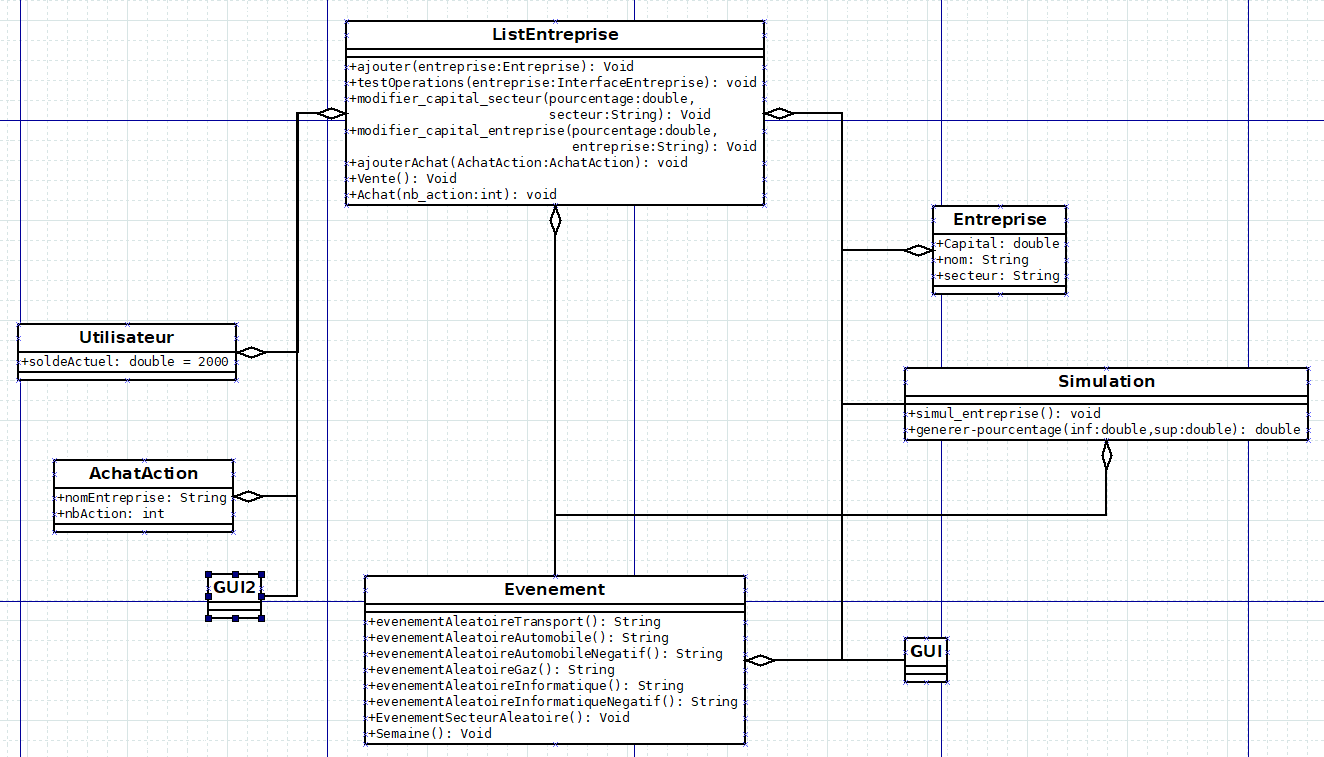
\includegraphics[width=3.5cm, height=2cm]{images/uml2.png}
%\caption{Diagramme UML}
%\label{fig:modele}
%\end{figure}

\fig{images/uml2.png}{19cm}{11.5cm}{Diagramme UML}{uml}

\subsection{Conception des classes de données}
\paragraph{} On a créer 2 classes 'objet' qui sont entreprise et utilisateur pour stocker les variables tels les capitaux, prix d'action, nom de l'entreprise, solde de l'utilisateur.

\paragraph{} Dans listEntreprise on a la création de l'arraylist contenant toute les entreprises ainsi que toutes les méthodes de manipulation d'entreprises pour modifier le capital/prix d'action ou encore faire des achats et ventes, on rappelle ses méthodes dans GUI et GUI2 ainsi que dans Evenement et simulation.
\paragraph{}Les classes simulation et Evenement contiennent les méthodes de modification de capital aléatoire par secteur ou par entreprise, les méthodes dans ces classes sont réutilisées dans GUI et GUI2.
\paragraph{}Les classes GUI et GUI2 correspondent à nos 2 fenêtres d'interface graphique, dans ses classes on rappelle les méthodes des autres classes ou on les modifie pour qu'elle soit affichables en interface graphique.
\paragraph{} 
\paragraph{} 
\subsection{Conception des traitements (processus)}
\paragraph{Le processus de notre projet consiste à chaque semaine :}
\begin{itemize}
\item De faire la simulation qui modifie entre -20 et +20 pourcent le capital de chaque entreprise.
\item Avoir un evenement aleatoire sur un secteur aléatoire.
\item Modifier le capital et le prix de l'action de chaque entreprise du secteur touché par l'evenement.
\item Achat/Vente si l'utilisateur le veut.
\end{itemize}
\paragraph{}On recommence le processus a chaque fois que l'utilisateur clique sur play


\subsection{Conception de l'IHM graphique}
\subsubsection{Première fenêtre}
\paragraph{Sur notre première fenêtre} On a la liste déroulante ou on choisis une entreprise pour soit la mettre en favori en cliquant sur "ajouter fav" ou l'afficher sur le graphique en cliquant sur "choisir entreprise". 
\paragraph{} Dans le graphique on affiche la fonction du prix d'action par rapport au temps (semaine par semaine) qui avance en cliquant play.
\paragraph{} Pour le graphique on utilise la librairie java.awt.graph et on utilise JButton pour les boutons play, ajouter fav et choisir entreprise.
\paragraph{} L'affichage des entreprises et news est fait grace a des JList.
\paragraph{}La liste des entreprises est fait avec un ListModel.

\paragraph{} Pour le graphique on a du utiliser la librairie externe JFreechart on a utiliser la commande createlineChart puis on a crée un DataSet pour stocker les valeurs a afficher dans le graphique.


%\begin{figure}
%\centering
%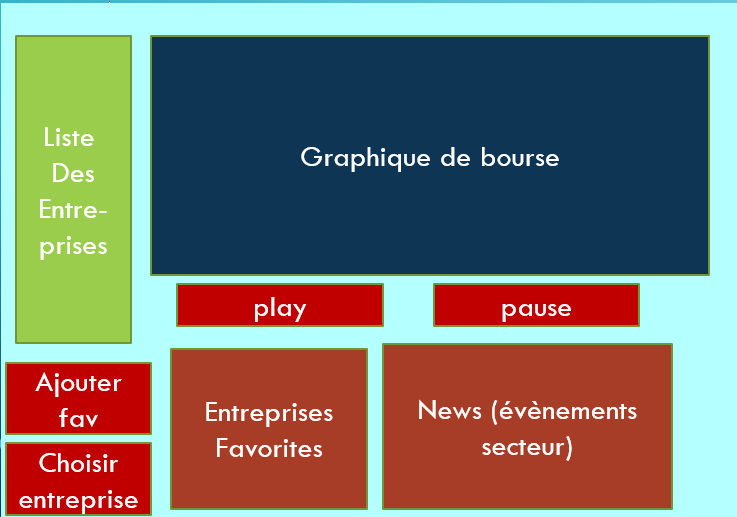
\includegraphics[width=3.5cm, height=2cm]{images/fenetre1.png}
%\caption{Première fenêtreL}
%\label{fig:modele}
%\end{figure}

\fig{images/fenetre1}{10.5cm}{7cm}{Première fenêtre}{Première fenêtre}


\paragraph{} 
\paragraph{} 
\paragraph{} 

\subsubsection{Deuxième fenêtre}
\paragraph{Sur notre deuxième fenêtre}on a crée des JList pour afficher les actions possédées et l'historique d'achat.
\paragraph{} On a ensuite une zone d'achat avec la liste deroulante des entreprises et une liste deroulante pour choisir le nombre d'action (JList) et un Jbutton pour valider l'achat d'action. 
\paragraph{} On a effectué de meme pour la partie vente.

%\begin{figure}
%\centering
%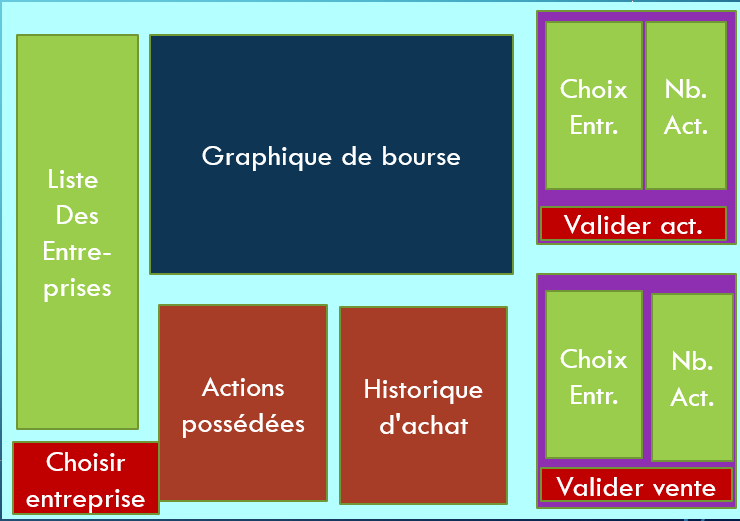
\includegraphics[width=3.5cm, height=2cm]{images/fenetre2.png}
%\caption{deuxième fenêtre}
%\label{fig:modele}
%\end{figure}

\fig{images/fenetre2.png}{10.5cm}{7cm}{deuxième fenêtre}{deuxième fenêtre}


\newpage
\section{Manuel utilisateur}
\label{sec:manuel}


\subsection{En ligne de commande}
\paragraph{} Pour tester nos méthode sans interface on clique sur "run" dans la classe Evenement qui va appeler toutes les classes necessaires a la simulation, l'achat et la vente d'action.
\paragraph{Dans un premier temps on aura l'affichage des informations sur les entreprises.}

%\begin{figure}
%\centering
%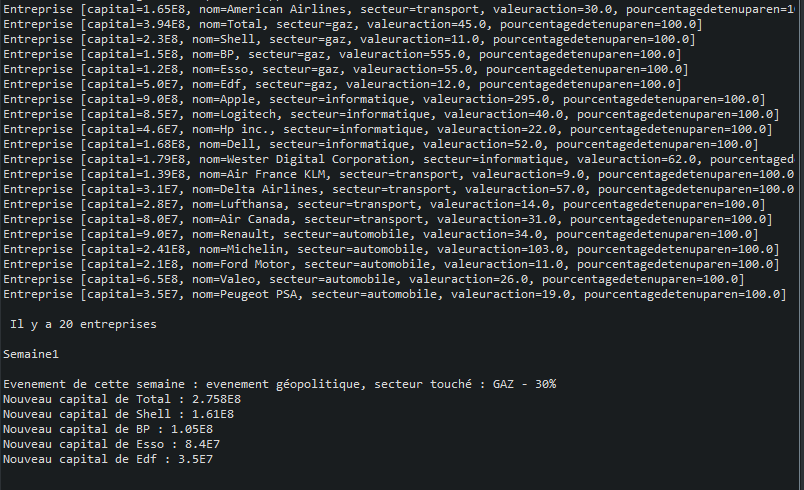
\includegraphics[width=3.5cm, height=2cm]{images/affichage1.png}
%\caption{Affichage CLI}
%\label{fig:modele}
%\end{figure}

\fig{images/affichage1.png}{12cm}{8cm}{Affichage CLI}{Affichage CLI}

\paragraph{]Ensuite on a le choix de faire un ou plusieurs achats/ventes, puis une nouvelle semaine commence.}

%\begin{figure}
%\centering
%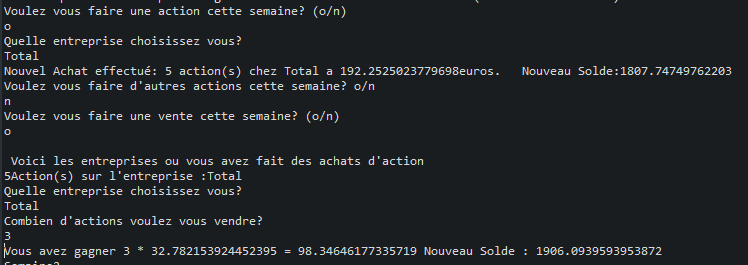
\includegraphics[width=3.5cm, height=2cm]{images/affichage2.png}
%\caption{Affichage CLI2}
%\label{fig:modele}
%\end{figure}

\fig{images/affichage2.png}{12cm}{4cm}{Affichage CLI2}{Affichage CLI2}

\paragraph{}
\paragraph{}
\paragraph{}
\paragraph{}

\subsection{En Interface graphique:}

\paragraph{}En interface graphique on a utilisé la librairie JFreeChart il faut donc installer les 2 fichiers jar jcommon-1.x.jar et jfreechart-1.x.jar telechargeable ici : \url{https://sourceforge.net/projects/jfreechart/} . Il faut ensuite placer les fichier dans un dossier lib dans le dossier source du projet.

\paragraph{}Ensuite dans eclipse il faut clic droit sur le dossier du projet, puis proprietés, Java build Path, librairies, cliquer sur classPath puis add Jar et aller dans le dossier lib pour choisir Jcommon, puis recommencer l'opération avec JFreechart.jar. 

%\begin{figure}
%\centering
%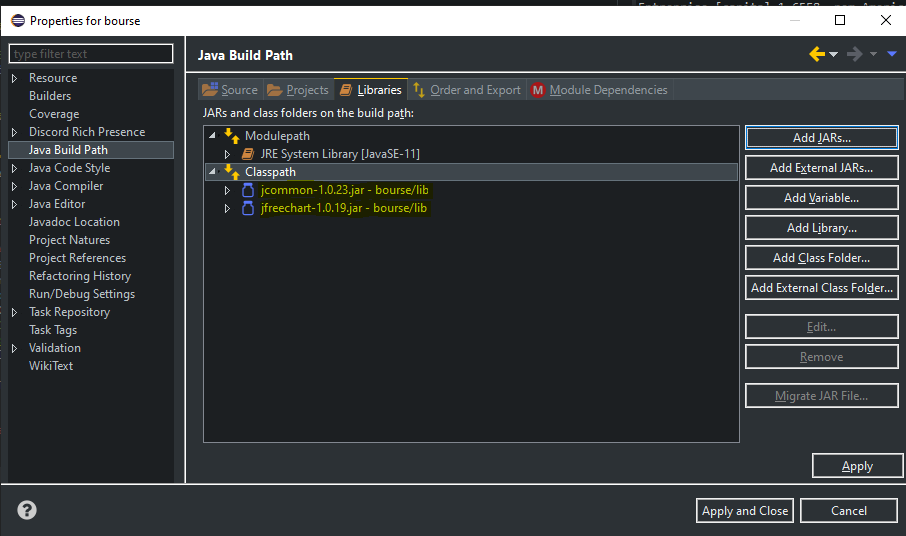
\includegraphics[width=3.5cm, height=2cm]{images/JFreechart.png}
%\caption{JFreechart}
%\label{fig:modele}
%\end{figure}

\fig{images/JFreechart.png}{13cm}{8.5cm}{JFreechart}{JFreechart}

\paragraph{}Ensuite on redemarre Eclipse.

\paragraph{} Pour lancer l'interface graphique, on clique sur "run" dans la classe GUI.

\paragraph{} On peut passer de la première a la deuxième fenêtre en cliquant sur le bouton haut de la fenêtre.

\paragraph{} Pour les fonctionnalités de l'interface elles sont assez simples a comprendre, on a juste a cliquer sur l'entreprise qu'on veut puis cliquer sur "choisir" pour l'afficher sur le graphique (cliquer sur la zone blanche du graphique si il ne s'affiche pas).
\paragraph{} En cliquant sur play une semaine passera et donc la zone news sera mise a jour.
\paragraph{} Sur la deuxième fenêtre pour vendre ou acheter des action on choisit son entreprise puis le nombre d'action et on clique sur "valider".


\newpage
\section{Déroulement du projet}
\label{sec:deroulement}

Dans cette section, nous décrivons comment le projet a été réalisé en équipe : la répartition des tâches, la synchronisation du travail en membres de l'équipe, etc.

\subsection{Réalisation du projet par étapes}
\paragraph{Voici les grandes étapes de conception de notre projet:}
\begin{enumerate}
\item Conception de l'UML de nos classes.
\item Programmation des classes de données tels Utilisateur Evenement et Entreprise.
\item Conception de nos 20 entreprises stockées dans une ArrayList.
\item Conception des evenements touchant des secteurs.
\item Conception de la classe listEntreprise pour manipuler notre ArrayList d'entreprise en la parcourant avec des iterator.
\item Schéma de nos deux fenêtres d'interface graphique.
\item Programmation du "squelette" de notre interface graphique.
\item Conception de la classe Simulation
\item Diaporama de presentation de projet.
\item  Mis en lien de nos classes de données et l'interface graphique.
\item Conception du graphique.
\item JavaDoc, rapport de projet, correction de nos classes.

\end{enumerate}

\subsection{Répartition des tâches entre membres de l'équipe}

\begin{tabular}{|*{13}{c|}}
    \hline
     / & 1 & 2  & 3  & 4  & 5  & 6  & 7  & 8  & 9  & 10 & 11 & 12 \\
    \hline
     Ayoub  & x  & x  &   &  & x &  &  & x & x &  & x & x\\
    \hline
     Hossein  & x  & x  &  & x & x &  &  & x & x &  &  &  \\
    \hline
     Julien  & x  &  & x &  &  & x & x &  &  & x & x & x \\
    \hline
\end{tabular}

\newpage
\section{Conclusion et perspectives}
\label{sec:conclusion}

\noindent Dans cette section, nous résumons la réalisation du projet et nous présentons également les extensions et améliorations possibles du projet.

\subsection{Résumé du travail réalisé}

\paragraph{}Ce projet nous a été très bénéfique tout d'abord dans l'aspect informatique : on a developpé nos connaissances en JAVA que ca soit en console avec les classes de données et de traitement avec la manipulation d'ArrayList avec un iterator ou en interface graphique ou on a manipulé differents elements d'affichage et de traitement.
\paragraph{}Le projet nous a aussi permis de mieux s'organiser en groupe car c'est plus compliqué de rassembler nos classes et de se répartir les taches a 3 alors qu'on est habituellement en binôme, on a donc dû utiliser des outils comme GitHub pour se partager nos fichiers ainsi que Discord pour s'appeler pendant le confinement et faire des partages d'écran.


\subsection{Améliorations possibles du projet}

\paragraph{}Pour améliorer le projet on pourrait ajouter les fonctionnalités avancées comme le swap, le future ou le forex.

\subsection{Sites et ressources utilisées}

\begin{itemize}
\item \url{https://stackoverflow.com/}
\item \url{https://www.java-forums.org/}
\item \url{https://www.vogella.com/tutorials/JFreeChart/article.html}
\item \url{https://docs.oracle.com/cd/E17802_01/j2se/javase/6/jcp/beta/apidiffs/java/sql/DataSet.html}
\item \url{https://www.boraji.com/jfreechart-xy-line-chart-example}
\item \url{https://openclassrooms.com/forum/}
\item \url{http://www.jfree.org/jfreechart/download.html}
\item \url{https://github.com/}
\end{itemize}




\end{document}
